\documentclass{book}

% ======== Packages ========
\usepackage[a4paper, top=2cm, bottom=3cm, left=2.5cm, right=2.5cm]{geometry}
\usepackage{titlesec}
\usepackage{tikz}
\usepackage{array}
\usepackage{xcolor}
\usepackage{etoolbox}
\usepackage[hidelinks]{hyperref}
\usepackage{lipsum}
\usepackage{lettrine}
\usepackage{listings}
\usepackage{inconsolata}
\usetikzlibrary{positioning, arrows.meta, shapes.geometric}

% ======== Custom Drop Cap Font (Zallman) ========
\usepackage{filecontents}
\begin{filecontents*}{Zallman.sty}
  \NeedsTeXFormat{LaTeX2e}
  \ProvidesPackage{Zallman}[2007/11/24 v1.0 Zallman CFR]
  \input Zallman.fd
  \DeclareRobustCommand{\Zallmanfamily}{
    \fontencoding{U}%
    \fontseries{xl}%
    \fontshape{n}%
    \fontfamily{Zallman}%
    \selectfont}
  \DeclareTextFontCommand{\zall}{\Zallmanfamily}
  \endinput
\end{filecontents*}
\usepackage{Zallman}
\renewcommand{\LettrineFontHook}{\color{Maroon}\Zallmanfamily}

% ======== Colors ========
\definecolor{deepred}{RGB}{153, 0, 0}
\definecolor{codebg}{RGB}{240,240,240}
\definecolor{codeborder}{RGB}{200,200,200}
\definecolor{keywordcolor}{RGB}{153, 0, 0}
\definecolor{Maroon}{RGB}{128, 0, 0}

% ======== Code Style ========
\lstdefinestyle{mystyle}{
  backgroundcolor=\color{codebg},
  basicstyle=\ttfamily\footnotesize,
  frame=single,
  rulecolor=\color{codeborder},
  keywordstyle=\color{keywordcolor}\bfseries,
  commentstyle=\color{gray},
  stringstyle=\color{blue},
  showstringspaces=false,
  breaklines=true,
  language=Python
}

% ======== Chapter spacing tweak ========
\makeatletter
\patchcmd{\@makechapterhead}{\vspace*{50\p@}}{\vspace*{10pt}}{}{}
\makeatother

% ======== Chapter style ========
\titleformat{\chapter}[display]
  {\normalfont\Large\bfseries}
  {\begin{tikzpicture}
      \fill[deepred] (0,0) rectangle (2,-2.8);
      \node[text=white, font=\small\bfseries, anchor=base] at (1,-0.3) {CHAPTER};
      \node[text=white, font=\fontsize{30}{36}\selectfont\bfseries] at (1,-1.5) {\thechapter};
    \end{tikzpicture}}
  {0.5em}
  {\MakeUppercase}
  [\vspace{0.3em}
   \small\itshape\mdseries\raggedleft
   "The true logic of this world is in the calculus of probabilities." \\
   \rule{\linewidth}{0.4pt} \\
   \textbf{--- James C. Maxwell}]
\titlespacing*{\chapter}{0pt}{0pt}{2em}

\titleformat{\section}
  {\normalfont\bfseries}
  {\thesection}
  {1em}{}

\titleformat{\subsection}
  {\normalfont\bfseries}
  {\thesubsection}
  {1em}{}

\newcolumntype{L}[1]{>{\raggedright\arraybackslash}p{#1}}
\newcolumntype{R}[1]{>{\raggedleft\arraybackslash}p{#1}}

% ======== Document starts ========
\begin{document}

% === COVER PAGE ===
\begin{titlepage}
\centering
\vspace*{3cm}
{\Huge\bfseries DEEP THINKING\par}
\vspace{0.5cm}
{\Large\itshape Notes on Learning Machines and the Human Mind\par}
\vspace{2cm}
{\LARGE\scshape Fauzy Madani\par}
\vfill
{\Large SMK Negeri 1 Garut \\ \texttt{fauzy\_madani@smknegeri1garut.sch.id}}
\vspace*{2cm}


\begin{tikzpicture}
  \draw[deepred, very thick] (0,0) rectangle (12,16);
  \node[anchor=south west, inner sep=0] (coverimg) at (0,0)
    {\includegraphics[width=12cm,height=16cm]{example-image}};
  \fill[white,opacity=0.8] (0,0) rectangle (12,16);
\end{tikzpicture}
\end{titlepage}
\clearpage

% === Author Page ===
\thispagestyle{empty}
\vspace*{5cm}
\begin{center}
  {\Huge\bfseries About the Author}

  \vspace{1cm}
  \lettrine[lines=3]{F}{auzy Madani} is not just a student of technology, but a contemplator of knowledge. He believes that understanding machines helps us understand ourselves — and that clarity is the highest form of empathy.

  \vspace{0.5cm}
  As a passionate software developer, his fascination lies in the overlap between artificial intelligence and human intuition, where logic meets mystery.

  \vspace{1cm}
  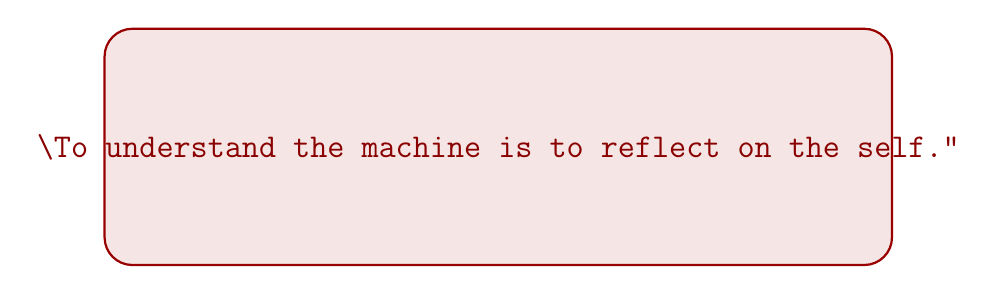
\begin{tikzpicture}
    \draw[deepred, thick, fill=deepred!10, rounded corners=10pt]
      (0,0) rectangle (10,3);
    \node[text=deepred!90!black, font=\large\ttfamily] at (5,1.5) {“To understand the machine is to reflect on the self.”};
  \end{tikzpicture}
\end{center}
\clearpage

% === Table of Contents ===
\tableofcontents
\clearpage

% === CHAPTER 1 ===
\chapter{How to Use This Book}

% Illustration
\begin{center}
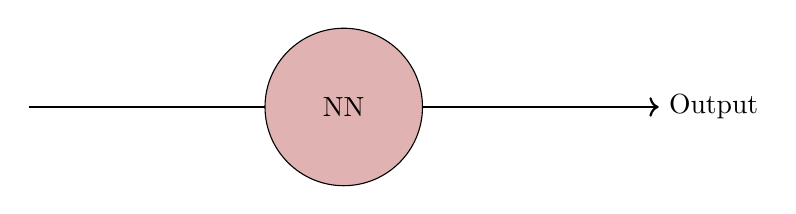
\begin{tikzpicture}
  \draw[->, thick] (0,0) -- (4,0) node[anchor=west] {Input};
  \draw[->, thick] (4,0) -- (8,0) node[anchor=west] {Output};
  \draw[fill=deepred!30] (4,0) circle (1);
  \node at (4,0) {NN};
\end{tikzpicture}

\vspace{0.5cm}
{\itshape Visual representation of a simple neural network.}
\end{center}

\section{Introduction}
\lettrine{F}{irst of all}, welcome to the world of Deep Learning Interviews. \lipsum[1]

\subsection{What makes this book so valuable}
\lettrine{D}{eciphering} dead languages. Detecting malignant tumours. Predicting natural disasters. \lipsum[2]

% === CHAPTER 2 ===
\chapter{Deep Learning Basics}

\section{What is a Neural Network?}
\lettrine{A}{rtificial} neurons are the building blocks. \lipsum[3]

\subsection{Perceptron}
\lettrine{T}{he} perceptron is a binary classifier. \lipsum[4]

\section{Training Deep Networks}
\subsection{Backpropagation}
\lettrine{B}{ackpropagation} is an essential technique. \lipsum[5]

% Complex Flowchart
\begin{center}
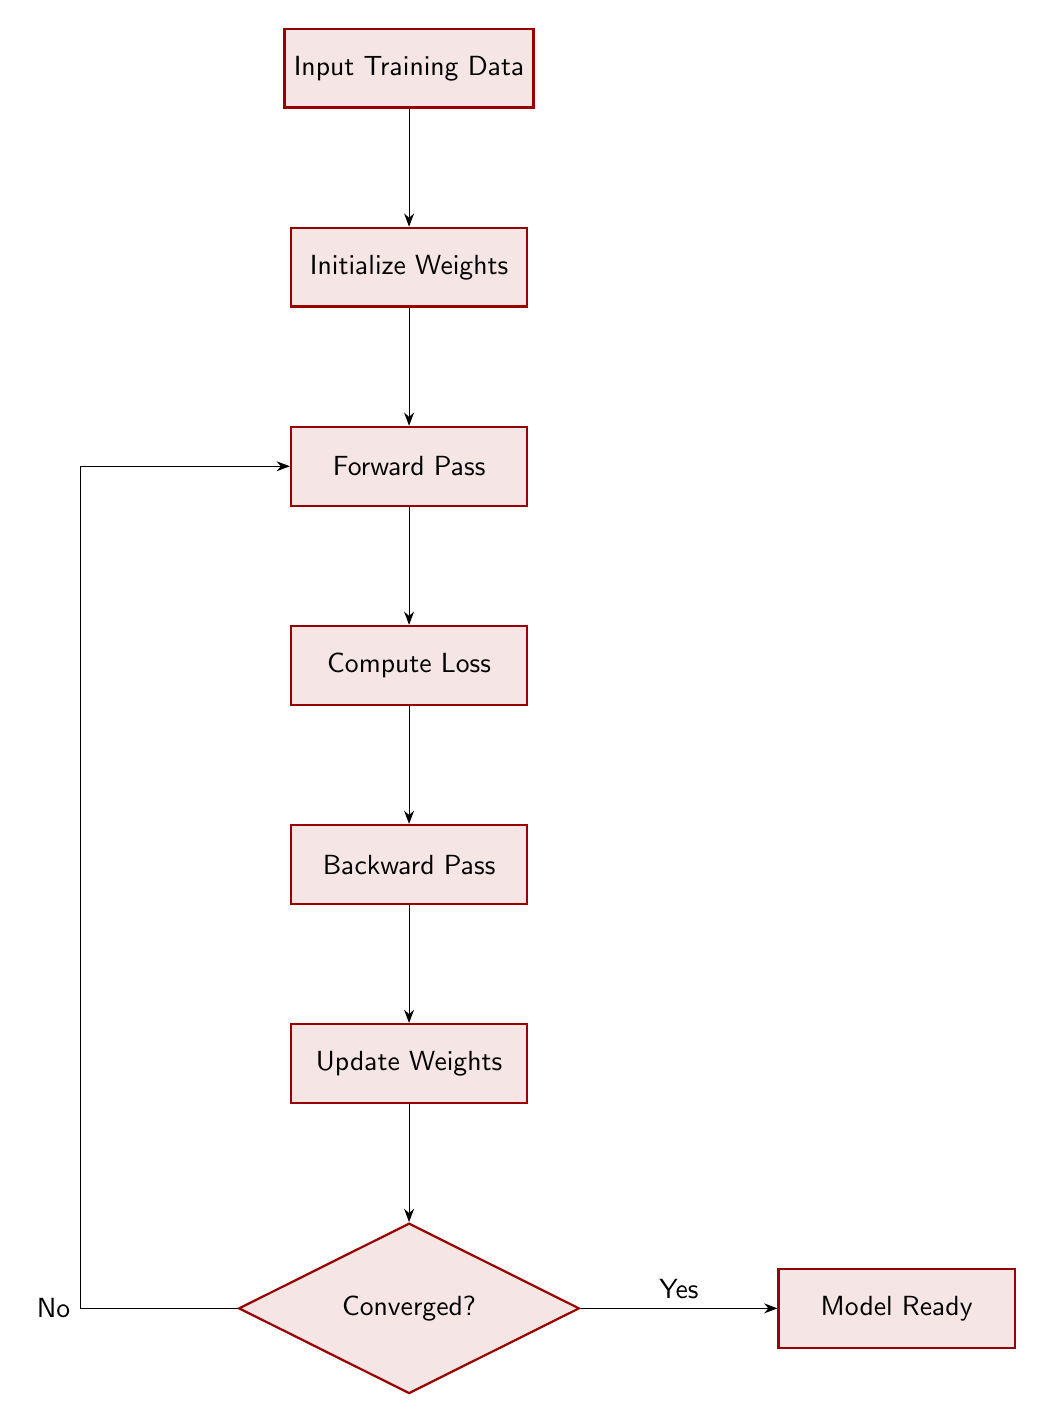
\begin{tikzpicture}[
  node distance=1.5cm and 2.5cm,
  every node/.style={font=\sffamily},
  process/.style={rectangle, draw=deepred, thick, fill=deepred!10, minimum width=3cm, minimum height=1cm},
  decision/.style={diamond, draw=deepred, thick, fill=deepred!10, aspect=2, text width=3cm, align=center},
  >=Stealth
]

\node[process] (data) {Input Training Data};
\node[process, below=of data] (init) {Initialize Weights};
\node[process, below=of init] (fwd) {Forward Pass};
\node[process, below=of fwd] (loss) {Compute Loss};
\node[process, below=of loss] (bwd) {Backward Pass};
\node[process, below=of bwd] (update) {Update Weights};
\node[decision, below=of update] (check) {Converged?};
\node[process, right=of check] (done) {Model Ready};

\draw[->] (data) -- (init);
\draw[->] (init) -- (fwd);
\draw[->] (fwd) -- (loss);
\draw[->] (loss) -- (bwd);
\draw[->] (bwd) -- (update);
\draw[->] (update) -- (check);
\draw[->] (check) -- node[above] {Yes} (done);
\draw[->] (check.west) -- ++(-2,0) node[left] {No} |- (fwd.west);

\end{tikzpicture}

\vspace{0.5cm}
{\itshape A more detailed training loop in a deep learning pipeline.}
\end{center}

\begin{lstlisting}[style=mystyle, caption={A simple neural net in PyTorch}]
import torch
import torch.nn as nn

class Net(nn.Module):
    def __init__(self):
        super(Net, self).__init__()
        self.fc = nn.Linear(10, 1)

    def forward(self, x):
        return self.fc(x)
\end{lstlisting}

% === CHAPTER 3 ===
\chapter{Advanced Topics}

\section{GANs and VAEs}
\lettrine{G}{enerative} models like GANs are powerful. \lipsum[6]

% === CHAPTER 4 ===
\chapter{Interview Questions}

\section{Theory}
\lettrine{T}{his} section covers theoretical concepts. \lipsum[7]

\section{Coding}
\lettrine{I}{nterviewers} often ask you to write code. \lipsum[8]

\end{document}

